\documentclass[11pt,letterpaper]{article}
\usepackage[margin=0.86in,top=0.82in,bottom=0.85in]{geometry}
\usepackage{booktabs,tabularx,array,graphicx,amsmath,xcolor,hyperref}
\usepackage{fancyhdr}
\definecolor{ink}{HTML}{1C313C}
\definecolor{teal}{HTML}{086964}
\definecolor{grey}{HTML}{4B6068}
\hypersetup{colorlinks=true,urlcolor=teal,linkcolor=teal,pdfauthor={Joseph Defendre},pdftitle={MORPH: Learning to Organize Computation in Neural Networks}}
\newcommand{\topic}[1]{\par\medskip\noindent\textbf{#1}\enspace}
\newcommand{\captext}[1]{{\small\color{grey}#1\par}}
\newcommand{\source}[2]{\href{#1}{#2}}
\setlength{\parindent}{0pt}
\setlength{\parskip}{5pt}
\renewcommand{\arraystretch}{1.15}
\setlength{\tabcolsep}{5.2pt}
\setlength{\emergencystretch}{2em}
\pagestyle{fancy}\fancyhf{}\fancyhead[L]{\small\color{grey}MORPH}\fancyhead[R]{\small\color{grey}Joseph Defendre}
\fancyfoot[R]{\small\color{grey}\thepage}\renewcommand{\headrulewidth}{0.2pt}
\begin{document}
\thispagestyle{plain}
{\sffamily\small\color{teal}RESEARCH REPORT\quad /\quad NOVEMBER 21, 2026}\par\vspace{6pt}
{\fontsize{27}{31}\selectfont\bfseries\raggedright\color{ink}MORPH: Learning to Organize\\Computation in Neural Networks\par}
\vspace{5pt}{\large Joseph Defendre}\par
\textit{Meta-Optimized Reconfigurable Processing Hierarchy}\par
\topic{Abstract.} Can a network learn to organize its computation more efficiently than a human-designed architecture? We tested input-dependent depth, grouping, expert routing and memory in eight experiments trained from scratch. On Boolean programs, adaptive depth reached 85.53\% accuracy and random depth 95.66\% at nearly identical estimated inference FLOPs. The clearest benefit came from choosing which information to retain and group. On a four-class synthetic task, grouping plus memory reached 100\% across three seeds. The full controller reached 91.17\%, and a policy written with knowledge of the task rules reached 99.84\%. Shuffling learned actions reduced full-model accuracy by 50.75 percentage points. Independent experiments recovered latent symbol families and retained relevant records under distribution shift. Uniform random expert routing matched learned routing on the task mixture. On natural text a five-minute, 118K-parameter decoder beat a smoothed bigram and generated dialogue-like bytes, yet it exited at one pass on every evaluated window. The experiments support several useful task-specific learned decisions. A general efficiency advantage of learning the entire computational organization remains unestablished.

\section*{1\quad What would count as evidence?}
A system that processes different inputs differently may still waste compute. We asked whether a trained policy can improve the accuracy available at a given cost, whether its decisions help the inputs receiving them, and whether those decisions survive a change in task difficulty. These are distinct empirical requirements. Comparing a model only with a deep, uniformly expensive baseline can reward an early exit even when a shallow network solves the task better.

We conducted eight experiments on one Apple M4 with 32 GiB of unified memory. Two recurrent Transformers implemented adaptive depth for reasoning and natural text. Separate component probes isolated grouping, routing and retention. A fourth benchmark implemented all four mechanisms together in a small recurrent classifier. Each predictor started from random initialization. The natural-language models learned depth alone. Results from the integrated classifier describe its synthetic task.

\topic{Protocol and comparisons.} Local, hashed or Git-versioned protocols fixed the targets before their respective runs. We report the initial runs and label the later investigations prompted by them. Three training seeds are the replication unit. Unless stated otherwise, brackets give descriptive two-sided, paired 95\% Student intervals with two degrees of freedom. These intervals can be wide and do not cover uncertainty over other datasets, task generators or machine types. We report both unfavorable and favorable outcomes.
\newpage
\section*{2\quad From halting probabilities to actual work}
Let $h_j$ be the recurrent state after pass $j$. The controller predicts a hazard $q_j=\sigma(g_\phi(h_j))$ for $j<4$ and sets $q_4=1$. The probability of stopping at $j$ and the training objective are
\[
p_j=q_j\prod_{i<j}(1-q_i),\qquad
L=\sum_{j=1}^4 p_j\bigl(\mathrm{CE}(y,f_\theta(h_j))+\lambda j\bigr).
\]
The relaxation computes all four possible exits during training. At inference the implementation applies a threshold, removes exited examples from the active batch and executes additional blocks only for survivors. A controller that exits at the same depth for every input implements a fixed inference policy.

\topic{Reasoning.} A causal decoder reads an initial bit, a random sequence of unary Boolean instructions interleaved with distractors, and a final query. The instructions copy, invert, set to zero or set to one. Chance accuracy is 50\%. Some reset instructions erase earlier dependencies, so the number of instructions measures nominal composition length. Training sequences have 32, 64 or 128 tokens and one to three instructions. All seven competitors for a seed receive the same training examples. Six controls comprise fixed recurrent depths one through four, uniform random recurrent depth, and a four-layer decoder with independent weights and reduced width to approximately match parameters. The adaptive model pays 0.012 nats per expected pass. On separate development data, its hard-exit threshold targets 2.5 passes; each resulting threshold is then frozen across test lengths.

\topic{Fair-cost frontier.} For each seed we maximize baseline accuracy subject to the adaptive model's estimated mean inference FLOPs. The comparison admits any input-independent mixture of two fixed policies. A cheap fixed policy dominates if it is already more accurate and fits under budget. Because frontier construction selects among fixed models using measured accuracies, the finite-test estimate can favor the baseline. The files also contain the individual fixed points and forced exits. Training equality is assessed separately against the shared four-pass model that processes identical examples and nearly identical arithmetic.

\topic{Measurement.} One matrix multiply-add counts as two FLOPs. Training estimates use three times the counted forward matrix operations. Dense-square attention estimates, filtering, synchronization, gates, tensor copies, optimizer work and memory bandwidth affect the relationship between these estimates and device time. Counts are specific to each implementation. The factorial benchmark reports linear multiply-adds (MACs). We do not combine its cost axis with Transformer FLOPs. Reported timings describe the reference hardware under shared load.

\topic{Distribution shifts and intervention.} The length-only test holds instruction counts in the training range and evaluates 256, 512 and 1,024 tokens. A separate test raises instruction counts to four through six at length 64. The ID set has 576 examples, the shifted sets 96 per condition. Reassigning the observed exits within each length preserves the marginal depth and estimated work and tests whether the original input received a particularly useful exit.
\newpage
\section*{3\quad Depth, interventions and extrapolation}
\topic{E1.} With 120 updates the 50,563-parameter adaptive model averaged 50.46\% in distribution. Its difference from the best fixed policy within budget was $-$6.71 [$-$29.88, +16.45] pp. The chance-level pilot motivated a separately frozen follow-up. All seven models were reinitialized, used new training and evaluation draws, and received 2,400 updates of 24 examples with learning-rate warmup, decay and clipping.
The untied 50,018-parameter decoder reached 98.78\% at 11.01 MFLOPs per input. Random depth reached 95.66\% at 23.30 MFLOPs. Adaptive reached 85.53\% at 23.38 MFLOPs. This last pair comes closest to an equal-cost direct comparison.
\begin{center}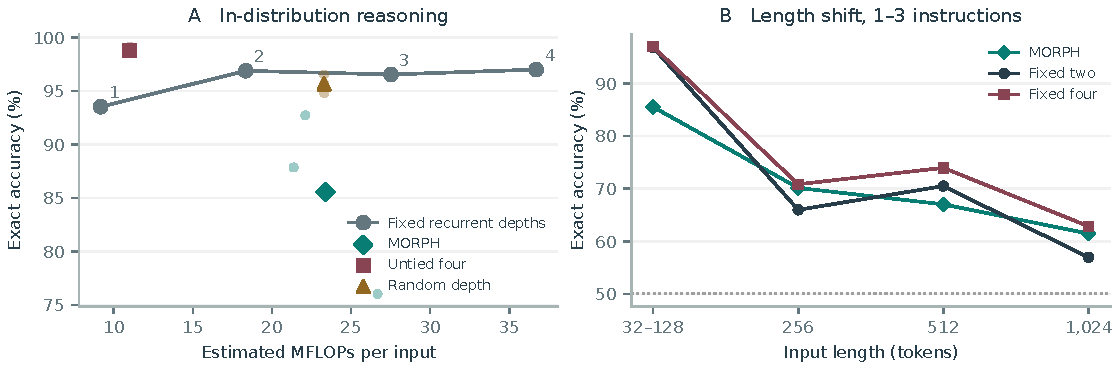
\includegraphics[width=.97\linewidth]{figures/reasoning.pdf}\end{center}
\captext{Figure 1. Mean of three paired seeds after longer training. Numbers mark fixed recurrent depths. Faint points at left are individual adaptive, random and untied seeds. ID lengths use 1--3 instructions.}
\begin{center}\small\begin{tabular}{lrrrr}\toprule
Test condition & MORPH, \% & Fixed two, \% & Passes & Gain vs. fixed frontier, pp\\\midrule
ID, 32--128 & 85.53 & 96.88 & 2.60 & $-$13.36 [$-$34.94, +8.22]\\
ID, 64 & 83.33 & 95.49 & 2.53 & $-$14.57 [$-$34.63, +5.48]\\
Length 256 & 70.14 & 65.97 & 2.03 & $-$8.33 [$-$19.61, +2.95]\\
Length 512 & 67.01 & 70.49 & 1.78 & $-$5.62 [$-$15.51, +4.27]\\
Length 1,024 & 61.46 & 56.94 & 1.54 & +1.53 [$-$8.51, +11.57]\\
4--6 ops, 64 & 84.03 & 94.10 & 2.50 & $-$10.07 [$-$17.97, $-$2.16]\\
\bottomrule\end{tabular}\end{center}
\topic{E6--7.} Reassigning the observed exits across inputs of the same length changed accuracy. The original-minus-shuffled difference on pooled ID examples was $-$2.33 [$-$19.96, +15.30] pp. Depth--instruction-count rank correlations were $-0.116$, $-0.019$ and $-0.071$ across seeds. Comparing the 64-token rows isolates instruction count. The longer rows change only length.
\topic{Qualification.} In a separate 8,000-update, seed-17 run on 14,293,248 token presentations, adaptive scored 1,087/1,152 (94.36\%) and fixed two scored 1,136/1,152 (98.61\%). Only fixed two passed the prespecified ID criterion. Their 1,024-token accuracies were 56.25\% and 65.63\%, respectively. Neither passed the shift criterion. Fixed two consumed 10.54 estimated training TFLOPs against 21.08 for adaptive.

\newpage
\section*{4\quad What the individual mechanisms learn}
\topic{E2. Grouping.} Sixteen observed symbol/value records precede a query. Twelve symbols have four hidden family identities, and each family shares a freshly sampled value within an episode. No family labels enter training. A writer maps records to slots and a learned reader predicts the query value. Only the query target contributes to the conditional perplexity (PPL) below. Random type assignments, adjacent segments and a fixed stride preserve the same number of slots.
\begin{center}
\begin{tabular}{rrrrrr}\toprule
Slots & Learned PPL & Random & Adjacent & Stride & Learned ARI\\\midrule
2 & 1.915 & 2.244 & 2.417 & 2.413 & 0.382\\
4 & 1.156 & 1.689 & 2.013 & 2.000 & 0.814\\
8 & 1.038 & 1.183 & 1.528 & 1.528 & 1.000\\\bottomrule
\end{tabular}
\end{center}
At four slots the learned writer reduced log loss by 0.377 nats against the strongest compressed control; the paired difference was $-0.377$ [$-0.802$, $+0.048$]. ARI is the label-invariant adjusted Rand index. Replacing the entire unseen suffix, including the answer, left the predictions unchanged. Four histogram slots used 256 bytes against 1,024 for sixteen slots of the same type. Sixteen packed raw records need only 32 bytes. The slot reduction does not establish physical memory savings against a compact representation.

\topic{E3. Experts.} Four two-layer experts learned modular addition, a bracket-stack query, copying and substitution from examples carrying task markers. Expected-risk top-one routing reached 100\% exact accuracy with 632 active parameters. Standard top-one routing reached 99.80\% with 632. Random routing reached 100\% with 556, and dense execution reached 100\% with 2,224. Learned-minus-standard accuracy was $+0.20$ percentage points (pp) [$-0.65$,$+1.04$]. Learned routes contained 0.234 bits of information about task identity. Cycling each choice to another expert reduced mean accuracy to 84.15\%. The finite task support admits interpolation, and uniform routing already solved the task.

\topic{E4. Retention.} An advance cue identifies which four colored records can be queried. At test the cue favors rare training colors and the relevant records move to the oldest quarter. With a four-entry limit and 32 input records, learned retention reached 100\%, uniform stride 18.26\% and a recent window 6.28\%. Randomly permuting learned priorities reduced recall to 18.15\%. Learned minus stride was $+81.74$ pp [79.62,83.85]. An explicit cue-matching rule also reached 100\%, using 12 cache bytes against 28 for learned retention, which also requires 325 model parameters.

A separately frozen follow-up used 1,024 records. Learned retention, cue matching and vectorized full attention recovered every query. Their retained arrays used 28, 12 and 3,072 bytes, respectively. Reference timings were 2,704, 60 and 66 microseconds per query. Python streaming versus vectorized dense execution strongly affects these timings. The experiment holds the number of relevant records fixed as the stream grows.
\newpage
\section*{5\quad Do the four mechanisms reinforce each other?}
\topic{E5. Factorial design.} A noisy four-dimensional header describes which bank of symbols to retain, which pair to combine, which transformation applies and how many repetitions the task requires. The model predicts one of four output classes. Header information is available before symbol storage begins. The controller receives answer supervision only. The design deliberately makes the computation choices identifiable and provides an informed human policy with access to the generator's rules.

All $2^4$ configurations and the human policy received 240 batches of 64 examples per seed. Every factorial cell averaged exactly two hard recurrent steps. Fixed cells use two steps for each input. Learned-depth cells assign one step to half of a 64-example cohort and three to the rest. All train through enumeration of possible paths. Hard inference executes a single choice at each decision. In the four-head accounting convention each factorial cell uses 1,568 linear MACs per prediction. Removing unused controller work gives deployment costs from 1,440 to 1,568.
\begin{center}
\begin{tabular}{lrr@{\qquad}lrr}\toprule
Cell & Accuracy & MACs & Cell & Accuracy & MACs\\\midrule
Fixed & 35.51\% & 1,440 & D+G & 57.82\% & 1,536\\
D & 36.21\% & 1,520 & D+R & 42.07\% & 1,536\\
G & 56.64\% & 1,520 & D+M & 57.39\% & 1,536\\
R & 41.68\% & 1,520 & G+M & 100.00\% & 1,536\\
M & 59.06\% & 1,520 & D+G+R+M & 91.17\% & 1,568\\
 & & & Informed policy & 99.84\% & 1,456\\\bottomrule
\end{tabular}
\end{center}
\captext{Mean of three training seeds on 4,096 shared examples. D = depth, G = grouping, R = expert routing, M = memory. MACs are the optimized linear arithmetic counts. The complete sixteen-cell table accompanies the paper.}

The registered full-model superadditivity contrast, $A_{DGRM}-\sum_i A_i+3A_0$, was $+4.09$ pp [$-5.90$,$+14.09$]. The six secondary pairwise contrasts were averaged over the remaining two factors. Grouping $\times$ memory yielded $+15.97$ pp [11.10,20.85], without adjustment for multiple comparisons. Grouping and memory together reached 100\% for all seeds and cost less than the full controller. A post-factorial static MLP received the complete input and used 1,556 MACs. At a matched estimated training budget it reached 30.18\% on 8,192 new cases, while grouping plus memory reached 100\%. The hand-designed policy remained highly competitive.

\topic{E6. Interventions.} Permuting full action tuples within cohorts preserved the joint histogram and reduced accuracy by 50.75 pp [32.93,68.57]. Permuting grouping alone cost 32.74 pp [23.42,42.06]; permuting memory alone cost 32.35 pp [23.94,40.76]. The depth-only effect was 4.13 pp [$-3.34$,$+11.61$]. Routing collapsed to one expert in two seeds. The evidence is strongest for which information is retained and combined.
\newpage
\section*{6\quad Does a depth advantage persist at scale?}
\topic{E8.} We widened the shared Boolean-program block to 896, 1,600 and 2,880 hidden dimensions. Every parameter belongs to an active computation or readout. The first ladder used 16 updates and 1,024 input token presentations per fit, with three paired seeds for fixed four and adaptive. It was a feasibility test. Training-time profiling motivated a second, separately registered 45-fit ladder with five independently trained models, three sizes and three seeds. Each fit received 160 updates, 1,280 examples and 40,960 input token presentations at length 32. The test used a new 256-example draw. The parameter count and training cost change together across sizes.
\begin{center}\small\begin{tabular}{lrrrrrr}\toprule
Params & MORPH, \% & Fixed 1 & Fixed 2 & Fixed 3 & Fixed 4 & Train TFLOPs\\\midrule
9.65M & 67.19 & 63.54 & 67.71 & 69.40 & 60.42 & 9.53\\
30.76M & 67.19 & 63.28 & 59.64 & 62.89 & 56.64 & 30.30\\
99.60M & 62.37 & 68.10 & 65.23 & 72.01 & 60.42 & 98.03\\
\bottomrule\end{tabular}\end{center}
\captext{Accuracy values are percentages on the controlled synthetic task. The last column is adaptive training arithmetic per fit. At each width the fixed-four model closely matches both the adaptive model's trainable parameters and its training arithmetic. Fixed one through four locate its inference frontier.}
\begin{center}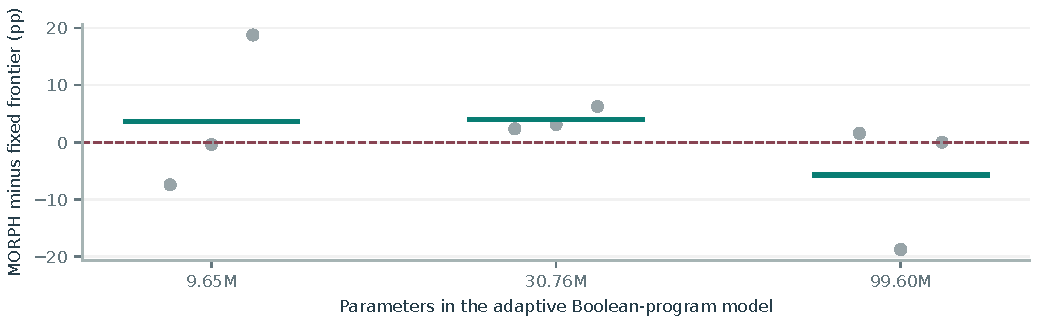
\includegraphics[width=.93\linewidth]{figures/scaling.pdf}\end{center}
\captext{Figure 2. Adaptive accuracy minus the best feasible fixed model or input-independent fixed mixture. Points are paired training seeds. Teal lines indicate means; zero indicates parity.}
\topic{Primary comparison.} The respective gains in percentage points at the three sizes were +3.65 [$-$30.00, +37.29], +3.91 [$-$1.23, +9.04], $-$5.73 [$-$33.81, +22.35]. On the original 16-update ladder adaptive accuracy was 46.88\%, 51.04\%, 50.00\%. Different test drawings and training schedules make the two ladders unsuitable for estimating a causal effect of training duration.
\topic{Calibration sensitivity.} Every scaled adaptive model chose one pass on every test case with the registered threshold grid. The three accuracy differences therefore cannot establish useful input-dependent depth. A post-hoc finer threshold search produced variation. Using only the original stored hazards, we calibrated on the first half of each archived test set and scored the second half. The gains against the fixed frontier at the three sizes were $-6.12$, $-2.97$ and $-7.78$ pp. Because this analysis was designed after the original tests, it is exploratory. Retraining discarded checkpoints changed some original-threshold predictions in five of twelve diagnostic records. The main tables use the original predictions. The companion data distinguish same-weight cached comparisons from retraining.


\newpage
\section*{7\quad A recurrent decoder trained on natural text}
We trained a byte-level language model on the first 892,315 bytes of the 1,115,394-byte Tiny Shakespeare corpus. The next tenth was reserved for validation and the final tenth for testing. Each 64-byte input predicts its final 48 next-byte targets. Held-out evaluation windows have disjoint scored targets. Training windows are sampled with replacement. Every context stays within its split. The test set contains 111,504 scored bytes. The adaptive policy reads the first 16 positions of the causal window and assigns one depth to its predicted suffix. Nothing after that prefix can affect the gate. \source{https://github.com/karpathy/char-rnn/tree/6f9487a6fe5b420b7ca9afb0d7c078e37c1d1b4e}{Pinned corpus source}.

\topic{Autoresearch.} Following Karpathy's validation-only keep/discard workflow, a 117,793-parameter MLX decoder received four 30-second development trials. The score combined validation bits per byte (BPB, lower is better) with 0.08 BPB per mean pass above two. We retained improvements exceeding 0.005. The baseline scored 2.554 and the successive candidates scored 2.879, 2.689 and 2.765. Reducing the pass penalty sent every window to depth four. The others exited at one. After three consecutive discards the stopping rule froze the baseline settings. A compile error before the first fit was logged separately. Under varying hardware contention, the baseline completed 5,228 updates and the final candidate 1,870. The trial order cannot identify the best hyperparameter at equal training progress.

\begin{center}\begin{tabular}{lrrrr}\toprule
118K model & Updates & BPB & Passes & Train TFLOPs\\\midrule
Fixed one & 320 & 3.796 & 1.00 & 0.242 \\
Fixed two & 320 & 3.701 & 2.00 & 0.447 \\
Fixed four & 320 & 3.697 & 4.00 & 0.858 \\
Random & 320 & 3.788 & 2.47 & 0.536 \\
MORPH & 320 & 3.694 & 1.00 & 0.966 \\
Fixed two, compute matched & 692 & 3.513 & 2.00 & 0.967 \\
\bottomrule\end{tabular}\end{center}
\captext{Three fresh seeds, one held-out segment. The compute-matched two-pass control received more byte presentations. Random training uses one depth per minibatch. Random evaluation draws per example. A pass of the 118K block uses about 13.37 million matrix FLOPs per 64-byte context before readout.}

The adaptive-minus-two-pass difference was $-0.007$ BPB [$-0.056$,$+0.042$]. At essentially equal inference arithmetic, the adaptive-training objective improved the one-pass result by 0.102 BPB. Each adaptive seed exited at one on every test window. Training through four exit losses can improve a shallow predictor even when it learns no input-dependent allocation. With nearly equal estimated training arithmetic, the two-pass control was better by 0.180 BPB [0.054,0.307]. Training on a larger number of windows is part of that comparison.

The smoothed bigram scored 3.625 BPB. An interpolated predictor with three prior bytes scored 2.908 BPB. The 320-update neural checkpoint failed the prespecified narrow utility margin of 0.10 BPB over bigram. The held-out test bytes belong to one corpus segment and the three training seeds share that segment.

\newpage
\section*{8\quad Longer training and usable checkpoints}
\topic{Repeat at equal progress.} A supplemental replay gave each of the four search configurations exactly 2,048 updates. Penalized validation BPB in the original trial order was 2.800, 3.159, 2.777 and 2.738. The original last-place learning rate now ranked first. We preserved the originally selected configuration for every subsequent test. A shared-device wall-clock search and a fixed-update experiment answer different questions.

\topic{External corpus.} We evaluated 154 Shakespeare sonnets from a pinned edition, excluding headers, footers and poem-crossing windows. The 1,828 windows contain 87,744 scored bytes. No exact full 65-byte window occurred in the training segment. Both corpora come from the same author. This is a change of work and genre within one author's English. \source{https://www.gutenberg.org/ebooks/1041}{The Sonnets, Project Gutenberg 1041}.
\begin{center}\begin{tabular}{lrrr}\toprule
4,096 updates, 118K & Plays BPB & Sonnets BPB & Sonnets passes\\\midrule
Fixed 1 & 3.074 & 2.846 & 1.00\\
Fixed 2 & 2.868 & 2.625 & 2.00\\
Fixed 4 & 2.870 & 2.588 & 4.00\\
MORPH & 2.875 & 2.598 & 1.00\\
\bottomrule\end{tabular}\end{center}
The prespecified longer-run adaptive-minus-fixed-two contrast on the sonnets was -0.027 [-0.153, +0.099] BPB. Each seed saw the same training windows across architectures. The play corpus had already been evaluated in the original comparison.


\topic{A five-minute checkpoint.} The separate seed-7 capstone completed 7,567 updates, 7.75 million input byte presentations and 22.85 estimated training TFLOPs in 300.02 seconds. The saved model achieved 2.789 BPB on the plays and 2.491 on the sonnets. The bigram achieved 3.625 and 3.480; the stronger three-byte-history model achieved 2.908 and 2.430, respectively. The capstone cleared the prespecified 0.10-BPB margin over bigram on both corpora. Its 117,793 trainable parameters fit in a checkpoint under 0.5 MB. It used exactly one recurrent pass on every evaluated input.

The model is usable for a byte-prediction experiment or a stylized text-generation demonstration. It can produce recognizable line breaks, character cues and invented words. The sample below begins with the fixed prompt and uses temperature 0.8 and sampling seed 73. Reloading the checkpoint reproduced the sample. We did not train a dialogue objective or measure instruction following.
\begin{quote}\small\ttfamily
To be, or not to be;\\
And I knersh well be thine will Aufide-shepher?\\[3pt]
ELBOHNOS:\\
I do my but offices me off the both,
\end{quote}

\newpage
\section*{9\quad A 30.32M-parameter language prototype}
We increased the hidden width to 1,728 and retained a single shared Transformer block with 16 attention heads. Matrix products use BF16 with FP32 master weights. The learned model has 30,321,217 trainable parameters. Fixed depths share 30,319,488 parameters and have identical starting backbone tensors for corresponding seeds. The three-seed comparison pairs 512 AdamW updates of four windows, or 131,072 input byte presentations per architecture and seed. The learning rate was 0.0003. Seed 11 continued to a prespecified 2,048 updates, totaling 524,288 input byte presentations. These budgets are small relative to the parameter count.

The original comparison trained fixed four and adaptive. A method-driven supplement trained fixed one and fixed two from scratch under the same data and update schedules. This closes a gap in interpreting shallow exits from weights optimized for four-pass execution. The supplement also evaluated seed 11 on the sonnets and checked the identity of the complete input arrays across versions of the data loader.\par
\begin{center}\small\begin{tabular}{lrrrr}\toprule
30M model & Plays, 512 & Passes, 512 & Plays, 2,048 & Sonnets, 2,048\\\midrule
Fixed 1 & 4.209 & 1.00 & 3.756 & 3.641\\
Fixed 2 & 4.197 & 2.00 & 3.740 & 3.628\\
Fixed 4 & 4.691 & 4.00 & 3.833 & ---\\
MORPH & 4.434 & 4.00 & 3.868 & 3.769\\
\bottomrule\end{tabular}\end{center}
\captext{Lower BPB is better. The 512-update plays results average three independent seeds. The 2,048-update endpoint uses seed 11 alone. The fixed-four Sonnets value was not measured.}


Fixed one, two and four used 3.893, 7.743 and 15.444 estimated inference GFLOPs per window. Training the expected loss at all adaptive exits consumed 4.00 times the arithmetic of fixed one, 2.01 times that of fixed two, and 1.008 times that of fixed four. Equal-step comparisons control data exposure; only fixed four closely matches the adaptive training budget.
\topic{At the observed budget.} On plays, the 512-update adaptive-minus-best-feasible-fixed BPB difference was +0.257 [-0.122, +0.636] across paired seeds. The descriptive envelope selects a fixed policy or mix at or below the measured cost on the same test set. At 2,048 updates the exported adaptive model scored 3.868 BPB at 4.00 mean passes. The 118K capstone saw substantially more data than this model. Size and training exposure are confounded in cross-size language comparisons.


\topic{A practical distinction.} A checkpoint can load, generate and score deterministically while still failing a useful comparison. The trained models with the clearest use cases here are the compact grouping-and-memory classifier on the specified inputs and the small byte predictor in the preceding section. On fresh in-distribution synthetic cases the classifier produced 9,999 correct predictions in 10,000 single-example calls. The two-pass Boolean classifier also qualified on its training-range task. The recorded inputs, command lines, seeds, local weights and results are supplied with the model card.

\newpage
\section*{10\quad Interpretation and prior work}
Adaptive depth has direct precedents. Graves learned recurrent halting and evaluated character-level language modeling. The Universal Transformer combined recurrent self-attention with adaptive halting. PonderNet optimized a distribution over stopping steps, while Mixture-of-Depths selected positions for computation under a budget. A 2026 preprint on token-selective attention directly includes Tiny Shakespeare. These designs and baselines make a first-invention claim for learned depth untenable. A matched comparison with their full implementations would be needed for a competitive methods paper. \source{https://arxiv.org/abs/1603.08983}{Graves (2016)}, \source{https://arxiv.org/abs/1807.03819}{Dehghani et al. (2019)}, \source{https://arxiv.org/abs/2107.05407}{Banino et al. (2021)}, \source{https://arxiv.org/abs/2404.02258}{Raposo et al. (2024)}, \source{https://arxiv.org/abs/2605.05222}{Mohammed (2026)}.

Conditional specialists have mature comparators in sparsely gated experts and Switch Transformers. Token Merging combines existing visual tokens, H-Net learns sequential chunking for byte-level language modeling, and HiT learns grouping and ungrouping for image diffusion. Dynamic Memory Compression learns cache compression in pretrained language models. Mixture of Nested Experts jointly varies token priority and expert compute. DARTS optimizes relaxed architecture choices during search. MORPH's deployed decisions also depend on each input. These methods address overlapping parts of the broader MORPH proposal under different architectures and tasks. This targeted literature check establishes relevant precedent. A systematic novelty review remains open. \source{https://arxiv.org/abs/1701.06538}{Shazeer et al. (2017)}, \source{https://arxiv.org/abs/2101.03961}{Fedus et al. (2022)}, \source{https://arxiv.org/abs/2210.09461}{Bolya et al. (2023)}, \source{https://arxiv.org/abs/2507.07955}{Hwang et al. (2025)}, \source{https://arxiv.org/abs/2611.22962}{Wu et al. (2026)}, \source{https://arxiv.org/abs/2403.09636}{Nawrot et al. (2024)}, \source{https://arxiv.org/abs/2407.19985}{Jain et al. (2024)}, \source{https://arxiv.org/abs/1806.09055}{Liu et al. (2019)}.

\topic{Scope of the evidence.} Three seeds distinguish catastrophic instability from consistent behavior in these runs, but have limited power for small effects. Some tasks deliberately provide a cue or task marker and repeatedly sample a finite input space. A loss surface that favors one exit can teach a controller to ignore its input. Targeting a mean depth on development data can restore variation without proving that the variation helps. This is why the shuffle interventions and strong fixed controls are central to interpretation. A 100M-parameter fit with few training tokens is evidence of engineering feasibility, with little bearing on language-model scaling at convergence.

\topic{Reproducibility and credit.} Joseph Defendre proposed MORPH, its research questions and the experimental roadmap. AI coding assistance implemented the experiments, ran the analyses and prepared this local manuscript. An independent clean-directory rerun reproduced all 285 main factorial and mechanism result rows on the checked scientific endpoints. The companion repository contains the frozen protocols, generator code, model weights, seed-level measurements, post-hoc extensions and reconstruction commands. The language loop adapts Andrej Karpathy's autoresearch procedure to Apple MLX. This report has not undergone external peer review. \source{https://github.com/karpathy/autoresearch/tree/228791fb499afffb54b46200aca536f79142f117}{Autoresearch source and revision}.
\end{document}
